\documentclass[10pt,a4paper]{article}
\usepackage[utf8]{inputenc}
\usepackage[T1]{fontenc}
\usepackage[spanish, es-tabla]{babel}

\usepackage{lmodern}
\usepackage{csquotes}

\usepackage{amsmath, amsfonts, amssymb, amsthm}
\usepackage{graphicx}

\usepackage[
    left=2.54cm,
    right=2.54cm,
    top=2.54cm,
    bottom=2.54cm
]{geometry}

\usepackage{tikz}
\usepackage{soul}
\usepackage{listings}

\usepackage[most]{tcolorbox}
\tcbset{shield externalize}

\usetikzlibrary{arrows.meta, positioning, automata}
\usetikzlibrary{babel}
\usetikzlibrary{external}
\tikzexternalize[prefix=build-tikz/]

\usepackage{xcolor}
\usepackage{hyperref}


\lstset{
    language=Python,
    basicstyle=\footnotesize\ttfamily,
    frame=single,
    numbers=left,
    inputencoding=utf8,
    extendedchars=true,
    breaklines=true,
    showstringspaces=false,
    keywordstyle=\color{blue},
    commentstyle=\color{green!50!black},
    stringstyle=\color{red!70!black}
}


\newtcbtheorem[number within=section]{ejercicio}{Ejercicio}{
    enhanced,
    sharp corners,
    boxrule=0pt,
    leftrule=5pt,
    colframe=gray!30!black,
    colback=gray!5!white,
    coltitle=white,
    fonttitle=\bfseries,
    separator sign={.\ },
    before skip=10pt,
    after skip=10pt
}{ej}

\newtcbtheorem[number within=section]{mytheo}{Teorema}{
    enhanced,
    sharp corners,
    boxrule=0pt,
    leftrule=5pt,
    colframe=blue!40!black,
    colback=blue!5!white,
    coltitle=white,
    fonttitle=\bfseries,
    separator sign={.\ },
    before skip=10pt,
    after skip=10pt
}{th}

\newtcolorbox{alerta}[1]{
    enhanced,
    sharp corners,
    boxrule=0pt,
    leftrule=5pt,
    colframe=red!40!black,
    colback=red!5!white,
    coltitle=white,
    fonttitle=\bfseries,
    title=#1,
    before skip=10pt,
    after skip=10pt
}

\newtcolorbox{nota}[1]{
    enhanced,
    sharp corners,
    boxrule=0pt,
    leftrule=5pt,
    colframe=orange!40!black,
    colback=yellow!5!white,
    coltitle=white,
    fonttitle=\bfseries,
    title=#1,
    before skip=10pt,
    after skip=10pt
}


\begin{document}

% PORTADA
\begin{titlepage}

    \centering

    {\huge \textbf{Universidad Nacional Autónoma de México}}\\[0.3cm]

    \rule{\linewidth}{2mm}\\[0.3cm]

    {\large \textbf{Facultad de Estudios Superiores Acatlán}}\\[1cm]

    
\includegraphics[width=6cm]{../../Archivos/LOGOS_IMG/acatlan.png}\\[1cm]

    {\Large \textbf{Matemáticas Aplicadas y Computación}}\\[1cm]

    {\huge \textbf{Sistemas Inteligentes}}\\[0.5cm]

    \rule{\linewidth}{1mm}\\[0.3cm]

    \vfill

    {\Large \textit{HILL CLIMBING}}\\[0.5cm]


    \vfill

    \rule{\linewidth}{0.5mm}\\[0.3cm]

    %{\Large \textit{Ricardo López Ramírez}}\\

    \rule{\linewidth}{0.5mm}\\[0.8cm]

    \small
    Actualización: \today \hfill Página: \thepage

\end{titlepage}


% ÍNDICE
\pagenumbering{roman}

\tableofcontents

\clearpage

\pagenumbering{arabic}

\setcounter{page}{1}

\section{Hill Climbing: Arad -> Bucarest}

El algoritmo Hill Climbing: Trazar el viaje de Arad a Bucarest.
Evaluar el valor \(h(n)\) de todos los vecinos generados y movernos solo al que tenga el 
valor más bajo.

Si en algún punto el mejor vecino tiene un valor \(h(n)\)  mayor o igual al de nodo actual
hemos llegado al \textbf{máximo local} y el algoritmo se detiene.

\vspace{3mm}


\begin{itemize}
    \item Estado Inicial:\\
    Nodo actual: Arad.\\
    \(h(n)\) actual: 366.

    \item Iteracion 1:\\
    Nodo actual: Arad.\\
    \(h(n)\) actual: 366.\\
    Vecinos evaluados: 
    \begin{itemize}
        \item Zerind (\(h=374\))
        \item Sibiu (\(h=253\))
        \item Timisoara (\(h=329\))
    \end{itemize}
    Decisión: Avanzar a Sibiu (\(253 < 366\)).

    \item Iteracion 2:\\
    Nodo actual: Sibiu.\\
    \(h(n)\) actual: 253.\\
    Vecinos evaluados: 
    \begin{itemize}
        \item Arad (\(h=366\))
        \item Oradea (\(h=380\))
        \item Fagaras (\(h=178\))
        \item Rimnicu Vilcea (\(h=193\))
    \end{itemize}
    Decisión: Avanzar a Fagaras (\(178 < 253\)).

    \item Iteracion 3:\\
    Nodo actual: Fagaras.\\
    \(h(n)\) actual: 178.\\
    Vecinos evaluados: 
    \begin{itemize}
        \item Sibiu (\(h=253\))
        \item Bucarest (\(h=0\))
    \end{itemize}
    Decisión: Avanzar a Bucarest (\(0 < 178\)).

    \item Iteracion 4:\\
    Nodo actual: Bucarest.\\
    \(h(n)\) actual: 0.\\
    Decisión: META ALCANZADA.

\end{itemize}


\begin{figure}[ht]
    \centering
    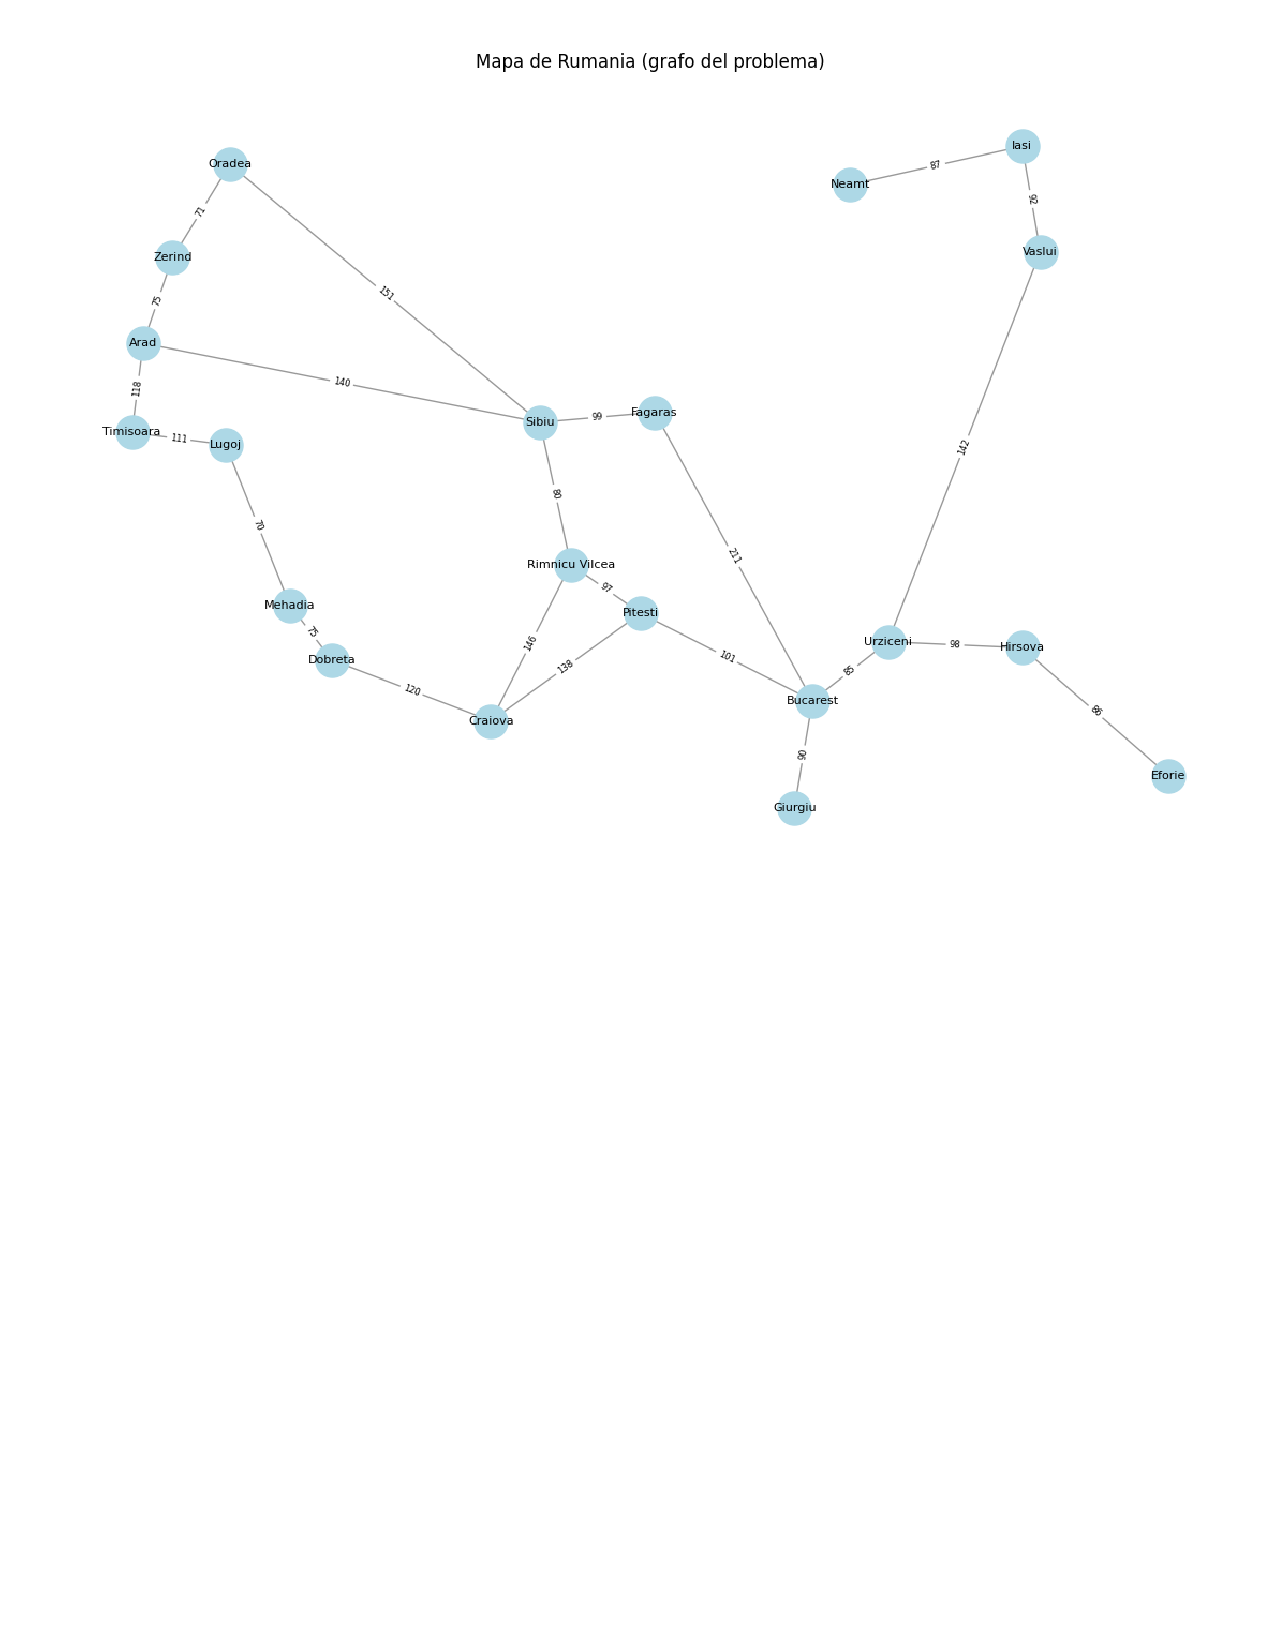
\includegraphics[width=0.8\textwidth]{../Actividad_4/Imagen/grafo.pdf}
    \caption{Documento adjunto.}
    \label{fig:documento}
\end{figure}


\end{document}